\documentclass[1p]{elsarticle_modified}
%\bibliographystyle{elsarticle-num}

%\usepackage[colorlinks]{hyperref}
%\usepackage{abbrmath_seonhwa} %\Abb, \Ascr, \Acal ,\Abf, \Afrak
\usepackage{amsfonts}
\usepackage{amssymb}
\usepackage{amsmath}
\usepackage{amsthm}
\usepackage{scalefnt}
\usepackage{amsbsy}
\usepackage{kotex}
\usepackage{caption}
\usepackage{subfig}
\usepackage{color}
\usepackage{graphicx}
\usepackage{xcolor} %% white, black, red, green, blue, cyan, magenta, yellow
\usepackage{float}
\usepackage{setspace}
\usepackage{hyperref}

\usepackage{tikz}
\usetikzlibrary{arrows}

\usepackage{multirow}
\usepackage{array} % fixed length table
\usepackage{hhline}

%%%%%%%%%%%%%%%%%%%%%
\makeatletter
\renewcommand*\env@matrix[1][\arraystretch]{%
	\edef\arraystretch{#1}%
	\hskip -\arraycolsep
	\let\@ifnextchar\new@ifnextchar
	\array{*\c@MaxMatrixCols c}}
\makeatother %https://tex.stackexchange.com/questions/14071/how-can-i-increase-the-line-spacing-in-a-matrix
%%%%%%%%%%%%%%%

\usepackage[normalem]{ulem}

\newcommand{\msout}[1]{\ifmmode\text{\sout{\ensuremath{#1}}}\else\sout{#1}\fi}
%SOURCE: \msout is \stkout macro in https://tex.stackexchange.com/questions/20609/strikeout-in-math-mode

\newcommand{\cancel}[1]{
	\ifmmode
	{\color{red}\msout{#1}}
	\else
	{\color{red}\sout{#1}}
	\fi
}

\newcommand{\add}[1]{
	{\color{blue}\uwave{#1}}
}

\newcommand{\replace}[2]{
	\ifmmode
	{\color{red}\msout{#1}}{\color{blue}\uwave{#2}}
	\else
	{\color{red}\sout{#1}}{\color{blue}\uwave{#2}}
	\fi
}

\newcommand{\Sol}{\mathcal{S}} %segment
\newcommand{\D}{D} %diagram
\newcommand{\A}{\mathcal{A}} %arc


%%%%%%%%%%%%%%%%%%%%%%%%%%%%%5 test

\def\sl{\operatorname{\textup{SL}}(2,\Cbb)}
\def\psl{\operatorname{\textup{PSL}}(2,\Cbb)}
\def\quan{\mkern 1mu \triangleright \mkern 1mu}

\theoremstyle{definition}
\newtheorem{thm}{Theorem}[section]
\newtheorem{prop}[thm]{Proposition}
\newtheorem{lem}[thm]{Lemma}
\newtheorem{ques}[thm]{Question}
\newtheorem{cor}[thm]{Corollary}
\newtheorem{defn}[thm]{Definition}
\newtheorem{exam}[thm]{Example}
\newtheorem{rmk}[thm]{Remark}
\newtheorem{alg}[thm]{Algorithm}

\newcommand{\I}{\sqrt{-1}}
\begin{document}

%\begin{frontmatter}
%
%\title{Boundary parabolic representations of knots up to 8 crossings}
%
%%% Group authors per affiliation:
%\author{Yunhi Cho} 
%\address{Department of Mathematics, University of Seoul, Seoul, Korea}
%\ead{yhcho@uos.ac.kr}
%
%
%\author{Seonhwa Kim} %\fnref{s_kim}}
%\address{Center for Geometry and Physics, Institute for Basic Science, Pohang, 37673, Korea}
%\ead{ryeona17@ibs.re.kr}
%
%\author{Hyuk Kim}
%\address{Department of Mathematical Sciences, Seoul National University, Seoul 08826, Korea}
%\ead{hyukkim@snu.ac.kr}
%
%\author{Seokbeom Yoon}
%\address{Department of Mathematical Sciences, Seoul National University, Seoul, 08826,  Korea}
%\ead{sbyoon15@snu.ac.kr}
%
%\begin{abstract}
%We find all boundary parabolic representation of knots up to 8 crossings.
%
%\end{abstract}
%\begin{keyword}
%    \MSC[2010] 57M25 
%\end{keyword}
%
%\end{frontmatter}

%\linenumbers
%\tableofcontents
%
\newcommand\colored[1]{\textcolor{white}{\rule[-0.35ex]{0.8em}{1.4ex}}\kern-0.8em\color{red} #1}%
%\newcommand\colored[1]{\textcolor{white}{ #1}\kern-2.17ex	\textcolor{white}{ #1}\kern-1.81ex	\textcolor{white}{ #1}\kern-2.15ex\color{red}#1	}

{\Large $\underline{11a_{283}~(K11a_{283})}$}

\setlength{\tabcolsep}{10pt}
\renewcommand{\arraystretch}{1.6}
\vspace{1cm}\begin{tabular}{m{100pt}>{\centering\arraybackslash}m{274pt}}
\multirow{5}{120pt}{
	\centering
	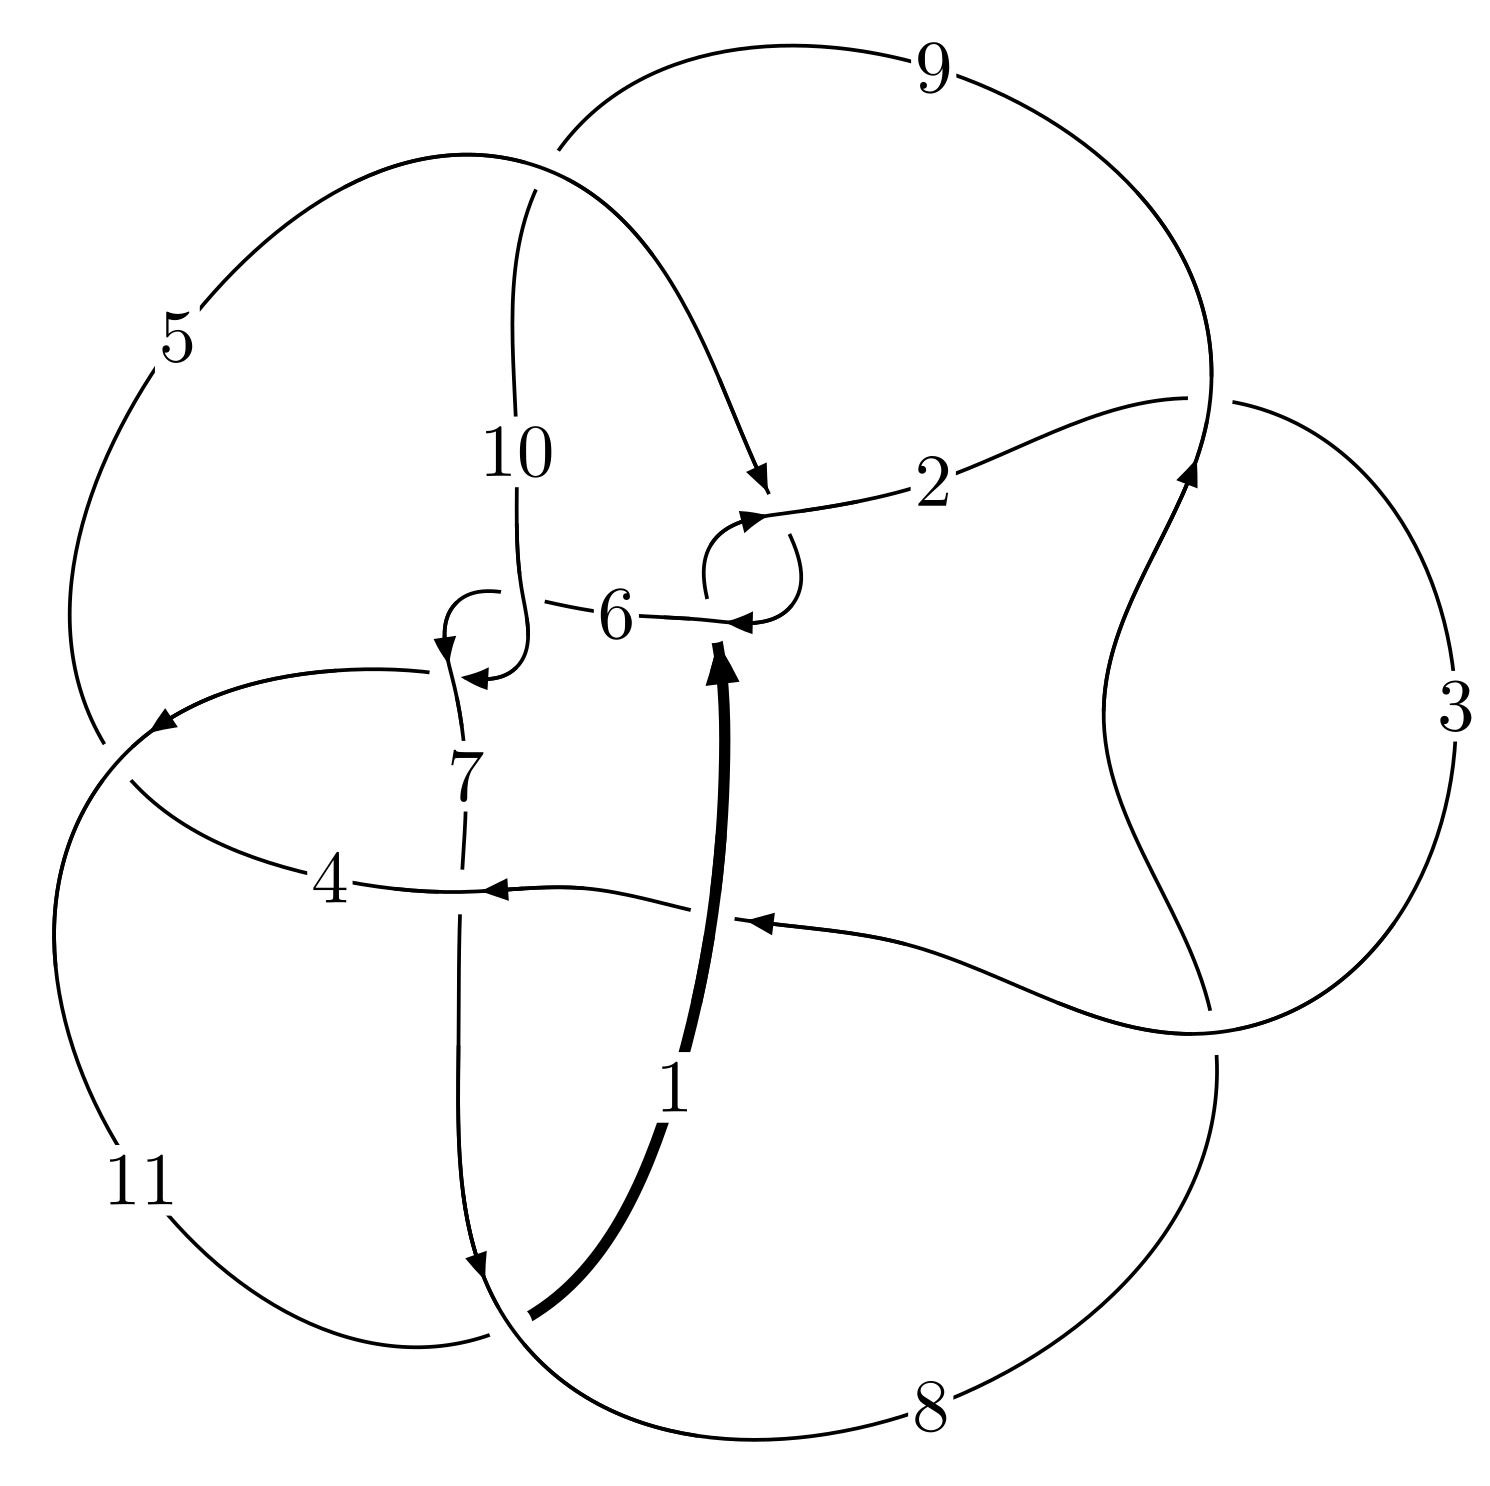
\includegraphics[width=112pt]{../../../GIT/diagram.site/Diagrams/png/532_11a_283.png}\\
\ \ \ A knot diagram\footnotemark}&
\allowdisplaybreaks
\textbf{Linearized knot diagam} \\
\cline{2-2}
 &
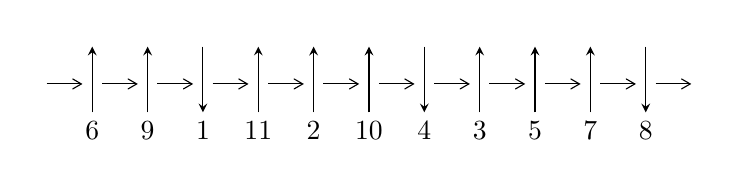
\begin{tikzpicture}[x=20pt, y=17pt]
	% nodes
	\node (C0) at (0, 0) {};
	\node (C1) at (1, 0) {};
	\node (C1U) at (1, +1) {};
	\node (C1D) at (1, -1) {6};

	\node (C2) at (2, 0) {};
	\node (C2U) at (2, +1) {};
	\node (C2D) at (2, -1) {9};

	\node (C3) at (3, 0) {};
	\node (C3U) at (3, +1) {};
	\node (C3D) at (3, -1) {1};

	\node (C4) at (4, 0) {};
	\node (C4U) at (4, +1) {};
	\node (C4D) at (4, -1) {11};

	\node (C5) at (5, 0) {};
	\node (C5U) at (5, +1) {};
	\node (C5D) at (5, -1) {2};

	\node (C6) at (6, 0) {};
	\node (C6U) at (6, +1) {};
	\node (C6D) at (6, -1) {10};

	\node (C7) at (7, 0) {};
	\node (C7U) at (7, +1) {};
	\node (C7D) at (7, -1) {4};

	\node (C8) at (8, 0) {};
	\node (C8U) at (8, +1) {};
	\node (C8D) at (8, -1) {3};

	\node (C9) at (9, 0) {};
	\node (C9U) at (9, +1) {};
	\node (C9D) at (9, -1) {5};

	\node (C10) at (10, 0) {};
	\node (C10U) at (10, +1) {};
	\node (C10D) at (10, -1) {7};

	\node (C11) at (11, 0) {};
	\node (C11U) at (11, +1) {};
	\node (C11D) at (11, -1) {8};
	\node (C12) at (12, 0) {};

	% arrows
	\draw[->,>={angle 60}]
	(C0) edge (C1) (C1) edge (C2) (C2) edge (C3) (C3) edge (C4) (C4) edge (C5) (C5) edge (C6) (C6) edge (C7) (C7) edge (C8) (C8) edge (C9) (C9) edge (C10) (C10) edge (C11) (C11) edge (C12) ;	\draw[->,>=stealth]
	(C1D) edge (C1U) (C2D) edge (C2U) (C3U) edge (C3D) (C4D) edge (C4U) (C5D) edge (C5U) (C6D) edge (C6U) (C7U) edge (C7D) (C8D) edge (C8U) (C9D) edge (C9U) (C10D) edge (C10U) (C11U) edge (C11D) ;
	\end{tikzpicture} \\
\hhline{~~} \\& 
\textbf{Solving Sequence} \\ \cline{2-2} 
 &
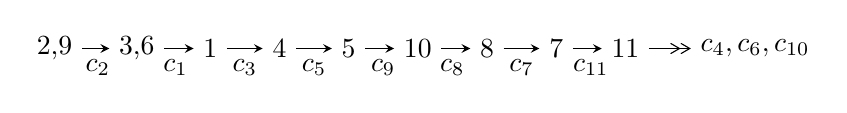
\begin{tikzpicture}[x=25pt, y=7pt]
	% node
	\node (A0) at (-1/8, 0) {2,9};
	\node (A1) at (17/16, 0) {3,6};
	\node (A2) at (17/8, 0) {1};
	\node (A3) at (25/8, 0) {4};
	\node (A4) at (33/8, 0) {5};
	\node (A5) at (41/8, 0) {10};
	\node (A6) at (49/8, 0) {8};
	\node (A7) at (57/8, 0) {7};
	\node (A8) at (65/8, 0) {11};
	\node (C1) at (1/2, -1) {$c_{2}$};
	\node (C2) at (13/8, -1) {$c_{1}$};
	\node (C3) at (21/8, -1) {$c_{3}$};
	\node (C4) at (29/8, -1) {$c_{5}$};
	\node (C5) at (37/8, -1) {$c_{9}$};
	\node (C6) at (45/8, -1) {$c_{8}$};
	\node (C7) at (53/8, -1) {$c_{7}$};
	\node (C8) at (61/8, -1) {$c_{11}$};
	\node (A9) at (10, 0) {$c_{4},c_{6},c_{10}$};

	% edge
	\draw[->,>=stealth]	
	(A0) edge (A1) (A1) edge (A2) (A2) edge (A3) (A3) edge (A4) (A4) edge (A5) (A5) edge (A6) (A6) edge (A7) (A7) edge (A8) ;
	\draw[->>,>={angle 60}]	
	(A8) edge (A9);
\end{tikzpicture} \\ 

\end{tabular} \\

\footnotetext{
The image of knot diagram is generated by the software ``\textbf{Draw programme}" developed by Andrew Bartholomew(\url{http://www.layer8.co.uk/maths/draw/index.htm\#Running-draw}), where we modified some parts for our purpose(\url{https://github.com/CATsTAILs/LinksPainter}).
}\phantom \\ \newline 
\centering \textbf{Ideals for irreducible components\footnotemark of $X_{\text{par}}$} 
 
\begin{align*}
I^u_{1}&=\langle 
-3.41985\times10^{252} u^{85}+4.09833\times10^{252} u^{84}+\cdots+1.22301\times10^{255} b-6.27945\times10^{254},\\
\phantom{I^u_{1}}&\phantom{= \langle  }-1.71138\times10^{256} u^{85}+1.63229\times10^{256} u^{84}+\cdots+1.02611\times10^{258} a+4.21212\times10^{259},\\
\phantom{I^u_{1}}&\phantom{= \langle  }u^{86}- u^{85}+\cdots-4313 u+839\rangle \\
I^u_{2}&=\langle 
6846 u^{19}-8204 u^{18}+\cdots+20003 b-10945,\\
\phantom{I^u_{2}}&\phantom{= \langle  }-1034553 u^{19}-1458425 u^{18}+\cdots+1180177 a-4013026,\;u^{20}+8 u^{18}+\cdots-3 u+1\rangle \\
I^u_{3}&=\langle 
u^2+b,\;a-1,\;u^7+u^5+u+1\rangle \\
\\
\end{align*}
\raggedright * 3 irreducible components of $\dim_{\mathbb{C}}=0$, with total 113 representations.\\
\footnotetext{All coefficients of polynomials are rational numbers. But the coefficients are sometimes approximated in decimal forms when there is not enough margin.}
\newpage
\renewcommand{\arraystretch}{1}
\centering \section*{I. $I^u_{1}= \langle -3.42\times10^{252} u^{85}+4.10\times10^{252} u^{84}+\cdots+1.22\times10^{255} b-6.28\times10^{254},\;-1.71\times10^{256} u^{85}+1.63\times10^{256} u^{84}+\cdots+1.03\times10^{258} a+4.21\times10^{259},\;u^{86}- u^{85}+\cdots-4313 u+839 \rangle$}
\flushleft \textbf{(i) Arc colorings}\\
\begin{tabular}{m{7pt} m{180pt} m{7pt} m{180pt} }
\flushright $a_{2}=$&$\begin{pmatrix}1\\0\end{pmatrix}$ \\
\flushright $a_{9}=$&$\begin{pmatrix}0\\u\end{pmatrix}$ \\
\flushright $a_{3}=$&$\begin{pmatrix}1\\- u^2\end{pmatrix}$ \\
\flushright $a_{6}=$&$\begin{pmatrix}0.0166784 u^{85}-0.0159077 u^{84}+\cdots+114.699 u-41.0496\\0.00279626 u^{85}-0.00335102 u^{84}+\cdots+16.6837 u+0.513442\end{pmatrix}$ \\
\flushright $a_{1}=$&$\begin{pmatrix}0.00695378 u^{85}-0.000700898 u^{84}+\cdots+21.3589 u+9.44845\\-0.0173378 u^{85}+0.0147297 u^{84}+\cdots-102.814 u+31.6226\end{pmatrix}$ \\
\flushright $a_{4}=$&$\begin{pmatrix}-0.00332478 u^{85}+0.000929287 u^{84}+\cdots-42.6202 u+8.23376\\0.00603896 u^{85}-0.00447428 u^{84}+\cdots+28.7233 u-4.85824\end{pmatrix}$ \\
\flushright $a_{5}=$&$\begin{pmatrix}0.0138821 u^{85}-0.0125566 u^{84}+\cdots+98.0158 u-41.5631\\0.00279626 u^{85}-0.00335102 u^{84}+\cdots+16.6837 u+0.513442\end{pmatrix}$ \\
\flushright $a_{10}=$&$\begin{pmatrix}-0.00463099 u^{85}-0.00234483 u^{84}+\cdots-22.7331 u-11.9767\\0.00886090 u^{85}-0.00901715 u^{84}+\cdots+82.5953 u-20.3806\end{pmatrix}$ \\
\flushright $a_{8}=$&$\begin{pmatrix}- u\\u^3+u\end{pmatrix}$ \\
\flushright $a_{7}=$&$\begin{pmatrix}0.00673940 u^{85}-0.00311584 u^{84}+\cdots+1.27697 u+5.88708\\0.00790831 u^{85}-0.0112601 u^{84}+\cdots+23.7107 u-8.85273\end{pmatrix}$ \\
\flushright $a_{11}=$&$\begin{pmatrix}0.0104754 u^{85}-0.00701084 u^{84}+\cdots+43.4674 u+6.56795\\-0.0169282 u^{85}+0.0130534 u^{84}+\cdots-109.942 u+32.1637\end{pmatrix}$\\ \flushright $a_{11}=$&$\begin{pmatrix}0.0104754 u^{85}-0.00701084 u^{84}+\cdots+43.4674 u+6.56795\\-0.0169282 u^{85}+0.0130534 u^{84}+\cdots-109.942 u+32.1637\end{pmatrix}$\\&\end{tabular}
\flushleft \textbf{(ii) Obstruction class $= -1$}\\~\\
\flushleft \textbf{(iii) Cusp Shapes $= -0.0966063 u^{85}+0.0534792 u^{84}+\cdots-636.168 u+175.613$}\\~\\
\newpage\renewcommand{\arraystretch}{1}
\flushleft \textbf{(iv) u-Polynomials at the component}\newline \\
\begin{tabular}{m{50pt}|m{274pt}}
Crossings & \hspace{64pt}u-Polynomials at each crossing \\
\hline $$\begin{aligned}c_{1},c_{5}\end{aligned}$$&$\begin{aligned}
&u^{86}-2 u^{85}+\cdots+4061 u+367
\end{aligned}$\\
\hline $$\begin{aligned}c_{2},c_{8}\end{aligned}$$&$\begin{aligned}
&u^{86}+u^{85}+\cdots+4313 u+839
\end{aligned}$\\
\hline $$\begin{aligned}c_{3}\end{aligned}$$&$\begin{aligned}
&u^{86}-10 u^{85}+\cdots-578 u+79
\end{aligned}$\\
\hline $$\begin{aligned}c_{4}\end{aligned}$$&$\begin{aligned}
&u^{86}-5 u^{85}+\cdots+16 u+1
\end{aligned}$\\
\hline $$\begin{aligned}c_{6},c_{10}\end{aligned}$$&$\begin{aligned}
&u^{86}+6 u^{85}+\cdots-2700 u+200
\end{aligned}$\\
\hline $$\begin{aligned}c_{7}\end{aligned}$$&$\begin{aligned}
&u^{86}+4 u^{85}+\cdots+379 u+169
\end{aligned}$\\
\hline $$\begin{aligned}c_{9}\end{aligned}$$&$\begin{aligned}
&u^{86}+u^{85}+\cdots+760266 u+130321
\end{aligned}$\\
\hline $$\begin{aligned}c_{11}\end{aligned}$$&$\begin{aligned}
&u^{86}+5 u^{85}+\cdots+690 u+179
\end{aligned}$\\
\hline
\end{tabular}\\~\\
\newpage\renewcommand{\arraystretch}{1}
\flushleft \textbf{(v) Riley Polynomials at the component}\newline \\
\begin{tabular}{m{50pt}|m{274pt}}
Crossings & \hspace{64pt}Riley Polynomials at each crossing \\
\hline $$\begin{aligned}c_{1},c_{5}\end{aligned}$$&$\begin{aligned}
&y^{86}+58 y^{85}+\cdots-1366917 y+134689
\end{aligned}$\\
\hline $$\begin{aligned}c_{2},c_{8}\end{aligned}$$&$\begin{aligned}
&y^{86}+73 y^{85}+\cdots-7899685 y+703921
\end{aligned}$\\
\hline $$\begin{aligned}c_{3}\end{aligned}$$&$\begin{aligned}
&y^{86}-14 y^{85}+\cdots-153964 y+6241
\end{aligned}$\\
\hline $$\begin{aligned}c_{4}\end{aligned}$$&$\begin{aligned}
&y^{86}-5 y^{85}+\cdots+200 y+1
\end{aligned}$\\
\hline $$\begin{aligned}c_{6},c_{10}\end{aligned}$$&$\begin{aligned}
&y^{86}-58 y^{85}+\cdots-4211600 y+40000
\end{aligned}$\\
\hline $$\begin{aligned}c_{7}\end{aligned}$$&$\begin{aligned}
&y^{86}+14 y^{85}+\cdots+1122169 y+28561
\end{aligned}$\\
\hline $$\begin{aligned}c_{9}\end{aligned}$$&$\begin{aligned}
&y^{86}+15 y^{85}+\cdots+56388593490 y+16983563041
\end{aligned}$\\
\hline $$\begin{aligned}c_{11}\end{aligned}$$&$\begin{aligned}
&y^{86}-19 y^{85}+\cdots-1161312 y+32041
\end{aligned}$\\
\hline
\end{tabular}\\~\\
\newpage\flushleft \textbf{(vi) Complex Volumes and Cusp Shapes}
$$\begin{array}{c|c|c}  
\text{Solutions to }I^u_{1}& \I (\text{vol} + \sqrt{-1}CS) & \text{Cusp shape}\\
 \hline 
\begin{aligned}
u &= -0.171045 + 0.950486 I \\
a &= \phantom{-}1.09878 + 2.26346 I \\
b &= \phantom{-}0.131608 + 0.877201 I\end{aligned}
 & \phantom{-}1.71658 + 1.70443 I & \phantom{-0.000000 } 0 \\ \hline\begin{aligned}
u &= -0.171045 - 0.950486 I \\
a &= \phantom{-}1.09878 - 2.26346 I \\
b &= \phantom{-}0.131608 - 0.877201 I\end{aligned}
 & \phantom{-}1.71658 - 1.70443 I & \phantom{-0.000000 } 0 \\ \hline\begin{aligned}
u &= -0.138042 + 1.039980 I \\
a &= \phantom{-}0.718636 + 0.240255 I \\
b &= -0.712835 + 0.801059 I\end{aligned}
 & \phantom{-}1.54553 - 2.70454 I & \phantom{-0.000000 } 0 \\ \hline\begin{aligned}
u &= -0.138042 - 1.039980 I \\
a &= \phantom{-}0.718636 - 0.240255 I \\
b &= -0.712835 - 0.801059 I\end{aligned}
 & \phantom{-}1.54553 + 2.70454 I & \phantom{-0.000000 } 0 \\ \hline\begin{aligned}
u &= -0.942410 + 0.113313 I \\
a &= \phantom{-}0.158648 + 0.099081 I \\
b &= \phantom{-}0.455331 + 1.100300 I\end{aligned}
 & \phantom{-}2.54751 + 4.69288 I & \phantom{-0.000000 } 0 \\ \hline\begin{aligned}
u &= -0.942410 - 0.113313 I \\
a &= \phantom{-}0.158648 - 0.099081 I \\
b &= \phantom{-}0.455331 - 1.100300 I\end{aligned}
 & \phantom{-}2.54751 - 4.69288 I & \phantom{-0.000000 } 0 \\ \hline\begin{aligned}
u &= \phantom{-}1.066980 + 0.013369 I \\
a &= \phantom{-}0.510040 - 0.562808 I \\
b &= -0.334819 - 1.068070 I\end{aligned}
 & -1.17731 + 3.15707 I & \phantom{-0.000000 } 0 \\ \hline\begin{aligned}
u &= \phantom{-}1.066980 - 0.013369 I \\
a &= \phantom{-}0.510040 + 0.562808 I \\
b &= -0.334819 + 1.068070 I\end{aligned}
 & -1.17731 - 3.15707 I & \phantom{-0.000000 } 0 \\ \hline\begin{aligned}
u &= \phantom{-}0.597375 + 0.937187 I \\
a &= \phantom{-}0.251462 + 0.325322 I \\
b &= \phantom{-}0.177390 - 0.920746 I\end{aligned}
 & \phantom{-}0.43505 + 5.35734 I & \phantom{-0.000000 } 0 \\ \hline\begin{aligned}
u &= \phantom{-}0.597375 - 0.937187 I \\
a &= \phantom{-}0.251462 - 0.325322 I \\
b &= \phantom{-}0.177390 + 0.920746 I\end{aligned}
 & \phantom{-}0.43505 - 5.35734 I & \phantom{-0.000000 } 0\\
 \hline 
 \end{array}$$\newpage$$\begin{array}{c|c|c}  
\text{Solutions to }I^u_{1}& \I (\text{vol} + \sqrt{-1}CS) & \text{Cusp shape}\\
 \hline 
\begin{aligned}
u &= \phantom{-}0.139913 + 1.108380 I \\
a &= -0.618464 + 0.196975 I \\
b &= -1.38818 + 0.35705 I\end{aligned}
 & \phantom{-}2.56807 + 2.29900 I & \phantom{-0.000000 } 0 \\ \hline\begin{aligned}
u &= \phantom{-}0.139913 - 1.108380 I \\
a &= -0.618464 - 0.196975 I \\
b &= -1.38818 - 0.35705 I\end{aligned}
 & \phantom{-}2.56807 - 2.29900 I & \phantom{-0.000000 } 0 \\ \hline\begin{aligned}
u &= -0.499950 + 1.009240 I \\
a &= \phantom{-}0.185257 - 0.499774 I \\
b &= \phantom{-}0.305862 + 0.044581 I\end{aligned}
 & -0.75390 - 3.34791 I & \phantom{-0.000000 } 0 \\ \hline\begin{aligned}
u &= -0.499950 - 1.009240 I \\
a &= \phantom{-}0.185257 + 0.499774 I \\
b &= \phantom{-}0.305862 - 0.044581 I\end{aligned}
 & -0.75390 + 3.34791 I & \phantom{-0.000000 } 0 \\ \hline\begin{aligned}
u &= -0.821993 + 0.102956 I \\
a &= -0.655973 + 0.796214 I \\
b &= \phantom{-}0.798776 + 0.329650 I\end{aligned}
 & \phantom{-}4.82477 - 6.81993 I & \phantom{-}10.08009 + 4.71115 I \\ \hline\begin{aligned}
u &= -0.821993 - 0.102956 I \\
a &= -0.655973 - 0.796214 I \\
b &= \phantom{-}0.798776 - 0.329650 I\end{aligned}
 & \phantom{-}4.82477 + 6.81993 I & \phantom{-}10.08009 - 4.71115 I \\ \hline\begin{aligned}
u &= -0.199723 + 1.160210 I \\
a &= -0.01752 - 3.29341 I \\
b &= \phantom{-}0.083947 - 0.961969 I\end{aligned}
 & \phantom{-}0.51451 - 6.45826 I & \phantom{-0.000000 } 0 \\ \hline\begin{aligned}
u &= -0.199723 - 1.160210 I \\
a &= -0.01752 + 3.29341 I \\
b &= \phantom{-}0.083947 + 0.961969 I\end{aligned}
 & \phantom{-}0.51451 + 6.45826 I & \phantom{-0.000000 } 0 \\ \hline\begin{aligned}
u &= -0.512127 + 0.559479 I \\
a &= \phantom{-}1.93509 - 0.19891 I \\
b &= -0.484188 - 0.707780 I\end{aligned}
 & \phantom{-}2.45089 + 3.89737 I & \phantom{-}6.40177 - 6.57898 I \\ \hline\begin{aligned}
u &= -0.512127 - 0.559479 I \\
a &= \phantom{-}1.93509 + 0.19891 I \\
b &= -0.484188 + 0.707780 I\end{aligned}
 & \phantom{-}2.45089 - 3.89737 I & \phantom{-}6.40177 + 6.57898 I\\
 \hline 
 \end{array}$$\newpage$$\begin{array}{c|c|c}  
\text{Solutions to }I^u_{1}& \I (\text{vol} + \sqrt{-1}CS) & \text{Cusp shape}\\
 \hline 
\begin{aligned}
u &= \phantom{-}0.057454 + 1.246560 I \\
a &= \phantom{-}0.37475 - 1.69448 I \\
b &= -0.60933 - 1.42722 I\end{aligned}
 & -7.29903 + 0.31589 I & \phantom{-0.000000 } 0 \\ \hline\begin{aligned}
u &= \phantom{-}0.057454 - 1.246560 I \\
a &= \phantom{-}0.37475 + 1.69448 I \\
b &= -0.60933 + 1.42722 I\end{aligned}
 & -7.29903 - 0.31589 I & \phantom{-0.000000 } 0 \\ \hline\begin{aligned}
u &= \phantom{-}0.412211 + 1.181190 I \\
a &= \phantom{-}0.60682 - 1.66020 I \\
b &= -0.23005 - 1.40830 I\end{aligned}
 & -4.58690 + 2.56469 I & \phantom{-0.000000 } 0 \\ \hline\begin{aligned}
u &= \phantom{-}0.412211 - 1.181190 I \\
a &= \phantom{-}0.60682 + 1.66020 I \\
b &= -0.23005 + 1.40830 I\end{aligned}
 & -4.58690 - 2.56469 I & \phantom{-0.000000 } 0 \\ \hline\begin{aligned}
u &= -0.163970 + 1.241080 I \\
a &= -1.07090 - 2.17182 I \\
b &= \phantom{-}0.44077 - 1.34783 I\end{aligned}
 & -4.48521 - 6.86672 I & \phantom{-0.000000 } 0 \\ \hline\begin{aligned}
u &= -0.163970 - 1.241080 I \\
a &= -1.07090 + 2.17182 I \\
b &= \phantom{-}0.44077 + 1.34783 I\end{aligned}
 & -4.48521 + 6.86672 I & \phantom{-0.000000 } 0 \\ \hline\begin{aligned}
u &= \phantom{-}1.203600 + 0.344486 I \\
a &= -0.387817 + 0.567429 I \\
b &= \phantom{-}0.500645 + 1.141340 I\end{aligned}
 & \phantom{-}2.30617 + 11.65450 I & \phantom{-0.000000 } 0 \\ \hline\begin{aligned}
u &= \phantom{-}1.203600 - 0.344486 I \\
a &= -0.387817 - 0.567429 I \\
b &= \phantom{-}0.500645 - 1.141340 I\end{aligned}
 & \phantom{-}2.30617 - 11.65450 I & \phantom{-0.000000 } 0 \\ \hline\begin{aligned}
u &= -0.662167 + 0.294205 I \\
a &= \phantom{-}0.461786 + 0.309921 I \\
b &= -0.610997 + 1.105130 I\end{aligned}
 & \phantom{-}2.64706 - 4.13307 I & \phantom{-}10.06650 + 7.67107 I \\ \hline\begin{aligned}
u &= -0.662167 - 0.294205 I \\
a &= \phantom{-}0.461786 - 0.309921 I \\
b &= -0.610997 - 1.105130 I\end{aligned}
 & \phantom{-}2.64706 + 4.13307 I & \phantom{-}10.06650 - 7.67107 I\\
 \hline 
 \end{array}$$\newpage$$\begin{array}{c|c|c}  
\text{Solutions to }I^u_{1}& \I (\text{vol} + \sqrt{-1}CS) & \text{Cusp shape}\\
 \hline 
\begin{aligned}
u &= \phantom{-}0.297470 + 1.255920 I \\
a &= -0.254293 - 0.144773 I \\
b &= -1.077280 - 0.185503 I\end{aligned}
 & -3.52274 + 6.07547 I & \phantom{-0.000000 } 0 \\ \hline\begin{aligned}
u &= \phantom{-}0.297470 - 1.255920 I \\
a &= -0.254293 + 0.144773 I \\
b &= -1.077280 + 0.185503 I\end{aligned}
 & -3.52274 - 6.07547 I & \phantom{-0.000000 } 0 \\ \hline\begin{aligned}
u &= \phantom{-}0.689327 + 0.123250 I \\
a &= \phantom{-}0.062912 + 1.059920 I \\
b &= \phantom{-}0.395529 + 0.164925 I\end{aligned}
 & \phantom{-}0.06236 - 2.46466 I & \phantom{-}6.83396 + 3.77647 I \\ \hline\begin{aligned}
u &= \phantom{-}0.689327 - 0.123250 I \\
a &= \phantom{-}0.062912 - 1.059920 I \\
b &= \phantom{-}0.395529 - 0.164925 I\end{aligned}
 & \phantom{-}0.06236 + 2.46466 I & \phantom{-}6.83396 - 3.77647 I \\ \hline\begin{aligned}
u &= \phantom{-}0.226747 + 1.282130 I \\
a &= -0.093690 - 0.200426 I \\
b &= \phantom{-}0.679000 - 0.036087 I\end{aligned}
 & -4.40326 + 0.41121 I & \phantom{-0.000000 } 0 \\ \hline\begin{aligned}
u &= \phantom{-}0.226747 - 1.282130 I \\
a &= -0.093690 + 0.200426 I \\
b &= \phantom{-}0.679000 + 0.036087 I\end{aligned}
 & -4.40326 - 0.41121 I & \phantom{-0.000000 } 0 \\ \hline\begin{aligned}
u &= -0.366588 + 1.260050 I \\
a &= \phantom{-}0.098420 - 0.273942 I \\
b &= \phantom{-}0.880454 + 0.085541 I\end{aligned}
 & -2.11426 - 4.00334 I & \phantom{-0.000000 } 0 \\ \hline\begin{aligned}
u &= -0.366588 - 1.260050 I \\
a &= \phantom{-}0.098420 + 0.273942 I \\
b &= \phantom{-}0.880454 - 0.085541 I\end{aligned}
 & -2.11426 + 4.00334 I & \phantom{-0.000000 } 0 \\ \hline\begin{aligned}
u &= -0.099264 + 1.314460 I \\
a &= \phantom{-}0.406154 + 0.976917 I \\
b &= \phantom{-}0.732172 + 0.382522 I\end{aligned}
 & \phantom{-}0.50203 + 2.48920 I & \phantom{-0.000000 } 0 \\ \hline\begin{aligned}
u &= -0.099264 - 1.314460 I \\
a &= \phantom{-}0.406154 - 0.976917 I \\
b &= \phantom{-}0.732172 - 0.382522 I\end{aligned}
 & \phantom{-}0.50203 - 2.48920 I & \phantom{-0.000000 } 0\\
 \hline 
 \end{array}$$\newpage$$\begin{array}{c|c|c}  
\text{Solutions to }I^u_{1}& \I (\text{vol} + \sqrt{-1}CS) & \text{Cusp shape}\\
 \hline 
\begin{aligned}
u &= \phantom{-}0.173406 + 1.315340 I \\
a &= -0.96739 + 1.70783 I \\
b &= \phantom{-}0.294787 + 1.239180 I\end{aligned}
 & -8.25891 + 3.00812 I & \phantom{-0.000000 } 0 \\ \hline\begin{aligned}
u &= \phantom{-}0.173406 - 1.315340 I \\
a &= -0.96739 - 1.70783 I \\
b &= \phantom{-}0.294787 - 1.239180 I\end{aligned}
 & -8.25891 - 3.00812 I & \phantom{-0.000000 } 0 \\ \hline\begin{aligned}
u &= -0.409443 + 1.263900 I \\
a &= \phantom{-}0.49046 + 1.63199 I \\
b &= -0.65824 + 1.38913 I\end{aligned}
 & -1.10942 - 9.46579 I & \phantom{-0.000000 } 0 \\ \hline\begin{aligned}
u &= -0.409443 - 1.263900 I \\
a &= \phantom{-}0.49046 - 1.63199 I \\
b &= -0.65824 - 1.38913 I\end{aligned}
 & -1.10942 + 9.46579 I & \phantom{-0.000000 } 0 \\ \hline\begin{aligned}
u &= \phantom{-}0.050986 + 1.328260 I \\
a &= \phantom{-}0.22173 + 1.98084 I \\
b &= -0.21254 + 1.53110 I\end{aligned}
 & -6.21226 + 5.37580 I & \phantom{-0.000000 } 0 \\ \hline\begin{aligned}
u &= \phantom{-}0.050986 - 1.328260 I \\
a &= \phantom{-}0.22173 - 1.98084 I \\
b &= -0.21254 - 1.53110 I\end{aligned}
 & -6.21226 - 5.37580 I & \phantom{-0.000000 } 0 \\ \hline\begin{aligned}
u &= \phantom{-}0.232857 + 1.345360 I \\
a &= -0.25117 + 2.15847 I \\
b &= \phantom{-}0.313690 + 1.368680 I\end{aligned}
 & -5.14196 + 5.75508 I & \phantom{-0.000000 } 0 \\ \hline\begin{aligned}
u &= \phantom{-}0.232857 - 1.345360 I \\
a &= -0.25117 - 2.15847 I \\
b &= \phantom{-}0.313690 - 1.368680 I\end{aligned}
 & -5.14196 - 5.75508 I & \phantom{-0.000000 } 0 \\ \hline\begin{aligned}
u &= -0.500434 + 0.387851 I \\
a &= \phantom{-}0.492345 + 0.241918 I \\
b &= -0.431811 + 0.295599 I\end{aligned}
 & \phantom{-}0.948430 - 0.603776 I & \phantom{-}9.01347 + 4.18465 I \\ \hline\begin{aligned}
u &= -0.500434 - 0.387851 I \\
a &= \phantom{-}0.492345 - 0.241918 I \\
b &= -0.431811 - 0.295599 I\end{aligned}
 & \phantom{-}0.948430 + 0.603776 I & \phantom{-}9.01347 - 4.18465 I\\
 \hline 
 \end{array}$$\newpage$$\begin{array}{c|c|c}  
\text{Solutions to }I^u_{1}& \I (\text{vol} + \sqrt{-1}CS) & \text{Cusp shape}\\
 \hline 
\begin{aligned}
u &= \phantom{-}0.042870 + 1.391350 I \\
a &= -0.08872 - 1.61352 I \\
b &= \phantom{-}0.455918 - 1.278250 I\end{aligned}
 & -6.14811 - 0.65193 I & \phantom{-0.000000 } 0 \\ \hline\begin{aligned}
u &= \phantom{-}0.042870 - 1.391350 I \\
a &= -0.08872 + 1.61352 I \\
b &= \phantom{-}0.455918 + 1.278250 I\end{aligned}
 & -6.14811 + 0.65193 I & \phantom{-0.000000 } 0 \\ \hline\begin{aligned}
u &= -0.359631 + 1.348720 I \\
a &= -0.470643 + 0.056389 I \\
b &= -1.242270 - 0.193872 I\end{aligned}
 & \phantom{-}0.23737 - 11.07660 I & \phantom{-0.000000 } 0 \\ \hline\begin{aligned}
u &= -0.359631 - 1.348720 I \\
a &= -0.470643 - 0.056389 I \\
b &= -1.242270 + 0.193872 I\end{aligned}
 & \phantom{-}0.23737 + 11.07660 I & \phantom{-0.000000 } 0 \\ \hline\begin{aligned}
u &= \phantom{-}0.596230 + 0.035731 I \\
a &= \phantom{-}0.684599 + 0.947731 I \\
b &= -0.411492 + 0.980008 I\end{aligned}
 & -0.80790 - 2.80909 I & \phantom{-}5.98332 - 0.21201 I \\ \hline\begin{aligned}
u &= \phantom{-}0.596230 - 0.035731 I \\
a &= \phantom{-}0.684599 - 0.947731 I \\
b &= -0.411492 - 0.980008 I\end{aligned}
 & -0.80790 + 2.80909 I & \phantom{-}5.98332 + 0.21201 I \\ \hline\begin{aligned}
u &= \phantom{-}0.417303 + 0.405708 I \\
a &= \phantom{-}0.14693 + 2.04390 I \\
b &= \phantom{-}0.765463 + 0.496537 I\end{aligned}
 & \phantom{-}4.56662 - 0.11637 I & \phantom{-}12.84009 - 2.25680 I \\ \hline\begin{aligned}
u &= \phantom{-}0.417303 - 0.405708 I \\
a &= \phantom{-}0.14693 - 2.04390 I \\
b &= \phantom{-}0.765463 - 0.496537 I\end{aligned}
 & \phantom{-}4.56662 + 0.11637 I & \phantom{-}12.84009 + 2.25680 I \\ \hline\begin{aligned}
u &= -0.26413 + 1.40109 I \\
a &= -0.28448 - 1.99461 I \\
b &= \phantom{-}0.66711 - 1.46071 I\end{aligned}
 & -2.71748 - 7.52821 I & \phantom{-0.000000 } 0 \\ \hline\begin{aligned}
u &= -0.26413 - 1.40109 I \\
a &= -0.28448 + 1.99461 I \\
b &= \phantom{-}0.66711 + 1.46071 I\end{aligned}
 & -2.71748 + 7.52821 I & \phantom{-0.000000 } 0\\
 \hline 
 \end{array}$$\newpage$$\begin{array}{c|c|c}  
\text{Solutions to }I^u_{1}& \I (\text{vol} + \sqrt{-1}CS) & \text{Cusp shape}\\
 \hline 
\begin{aligned}
u &= \phantom{-}0.10686 + 1.50124 I \\
a &= -0.245884 + 1.141140 I \\
b &= \phantom{-}0.783069 + 1.067070 I\end{aligned}
 & -5.72875 + 3.11452 I & \phantom{-0.000000 } 0 \\ \hline\begin{aligned}
u &= \phantom{-}0.10686 - 1.50124 I \\
a &= -0.245884 - 1.141140 I \\
b &= \phantom{-}0.783069 - 1.067070 I\end{aligned}
 & -5.72875 - 3.11452 I & \phantom{-0.000000 } 0 \\ \hline\begin{aligned}
u &= -0.22724 + 1.49618 I \\
a &= -0.81530 - 1.31196 I \\
b &= -0.020931 - 0.994862 I\end{aligned}
 & -3.17742 + 0.08844 I & \phantom{-0.000000 } 0 \\ \hline\begin{aligned}
u &= -0.22724 - 1.49618 I \\
a &= -0.81530 + 1.31196 I \\
b &= -0.020931 + 0.994862 I\end{aligned}
 & -3.17742 - 0.08844 I & \phantom{-0.000000 } 0 \\ \hline\begin{aligned}
u &= \phantom{-}0.54898 + 1.41093 I \\
a &= -0.82747 + 1.53406 I \\
b &= \phantom{-}0.517955 + 1.251330 I\end{aligned}
 & -5.61570 + 9.08985 I & \phantom{-0.000000 } 0 \\ \hline\begin{aligned}
u &= \phantom{-}0.54898 - 1.41093 I \\
a &= -0.82747 - 1.53406 I \\
b &= \phantom{-}0.517955 - 1.251330 I\end{aligned}
 & -5.61570 - 9.08985 I & \phantom{-0.000000 } 0 \\ \hline\begin{aligned}
u &= -1.41382 + 0.54274 I \\
a &= -0.150367 - 0.669536 I \\
b &= \phantom{-}0.207903 - 1.033730 I\end{aligned}
 & -2.09582 - 4.89045 I & \phantom{-0.000000 } 0 \\ \hline\begin{aligned}
u &= -1.41382 - 0.54274 I \\
a &= -0.150367 + 0.669536 I \\
b &= \phantom{-}0.207903 + 1.033730 I\end{aligned}
 & -2.09582 + 4.89045 I & \phantom{-0.000000 } 0 \\ \hline\begin{aligned}
u &= -0.68545 + 1.36638 I \\
a &= \phantom{-}0.30951 + 1.38848 I \\
b &= -0.088050 + 0.737680 I\end{aligned}
 & \phantom{-}1.18894 + 2.12493 I & \phantom{-0.000000 } 0 \\ \hline\begin{aligned}
u &= -0.68545 - 1.36638 I \\
a &= \phantom{-}0.30951 - 1.38848 I \\
b &= -0.088050 - 0.737680 I\end{aligned}
 & \phantom{-}1.18894 - 2.12493 I & \phantom{-0.000000 } 0\\
 \hline 
 \end{array}$$\newpage$$\begin{array}{c|c|c}  
\text{Solutions to }I^u_{1}& \I (\text{vol} + \sqrt{-1}CS) & \text{Cusp shape}\\
 \hline 
\begin{aligned}
u &= \phantom{-}0.48985 + 1.50866 I \\
a &= \phantom{-}0.52759 - 1.65020 I \\
b &= -0.63184 - 1.35216 I\end{aligned}
 & -3.4892 + 17.6295 I & \phantom{-0.000000 } 0 \\ \hline\begin{aligned}
u &= \phantom{-}0.48985 - 1.50866 I \\
a &= \phantom{-}0.52759 + 1.65020 I \\
b &= -0.63184 + 1.35216 I\end{aligned}
 & -3.4892 - 17.6295 I & \phantom{-0.000000 } 0 \\ \hline\begin{aligned}
u &= \phantom{-}0.386003 + 0.111568 I \\
a &= \phantom{-}0.72617 - 1.21676 I \\
b &= -1.015930 - 0.376348 I\end{aligned}
 & \phantom{-}4.95207 + 1.65937 I & \phantom{-}17.2147 - 3.6067 I \\ \hline\begin{aligned}
u &= \phantom{-}0.386003 - 0.111568 I \\
a &= \phantom{-}0.72617 + 1.21676 I \\
b &= -1.015930 + 0.376348 I\end{aligned}
 & \phantom{-}4.95207 - 1.65937 I & \phantom{-}17.2147 + 3.6067 I \\ \hline\begin{aligned}
u &= -0.48750 + 1.53880 I \\
a &= \phantom{-}0.43487 + 1.58941 I \\
b &= -0.44392 + 1.36956 I\end{aligned}
 & -8.42324 - 11.27470 I & \phantom{-0.000000 } 0 \\ \hline\begin{aligned}
u &= -0.48750 - 1.53880 I \\
a &= \phantom{-}0.43487 - 1.58941 I \\
b &= -0.44392 - 1.36956 I\end{aligned}
 & -8.42324 + 11.27470 I & \phantom{-0.000000 } 0 \\ \hline\begin{aligned}
u &= \phantom{-}1.29645 + 0.97439 I \\
a &= -0.150528 + 0.680017 I \\
b &= -0.180507 + 0.936717 I\end{aligned}
 & \phantom{-}0.43071 - 3.88005 I & \phantom{-0.000000 } 0 \\ \hline\begin{aligned}
u &= \phantom{-}1.29645 - 0.97439 I \\
a &= -0.150528 - 0.680017 I \\
b &= -0.180507 - 0.936717 I\end{aligned}
 & \phantom{-}0.43071 + 3.88005 I & \phantom{-0.000000 } 0 \\ \hline\begin{aligned}
u &= \phantom{-}0.360463 + 0.104511 I \\
a &= \phantom{-}1.71701 + 1.38281 I \\
b &= \phantom{-}0.099604 - 1.152090 I\end{aligned}
 & -3.81257 + 0.89485 I & -2.25949 - 1.18834 I \\ \hline\begin{aligned}
u &= \phantom{-}0.360463 - 0.104511 I \\
a &= \phantom{-}1.71701 - 1.38281 I \\
b &= \phantom{-}0.099604 + 1.152090 I\end{aligned}
 & -3.81257 - 0.89485 I & -2.25949 + 1.18834 I\\
 \hline 
 \end{array}$$\newpage$$\begin{array}{c|c|c}  
\text{Solutions to }I^u_{1}& \I (\text{vol} + \sqrt{-1}CS) & \text{Cusp shape}\\
 \hline 
\begin{aligned}
u &= \phantom{-}0.67498 + 1.51204 I \\
a &= \phantom{-}0.37015 - 1.38509 I \\
b &= -0.106244 - 1.278550 I\end{aligned}
 & -5.01653 + 3.29033 I & \phantom{-0.000000 } 0 \\ \hline\begin{aligned}
u &= \phantom{-}0.67498 - 1.51204 I \\
a &= \phantom{-}0.37015 + 1.38509 I \\
b &= -0.106244 + 1.278550 I\end{aligned}
 & -5.01653 - 3.29033 I & \phantom{-0.000000 } 0 \\ \hline\begin{aligned}
u &= -0.46654 + 1.63346 I \\
a &= -0.45448 - 1.42613 I \\
b &= \phantom{-}0.380524 - 1.198130 I\end{aligned}
 & -7.86731 - 4.29450 I & \phantom{-0.000000 } 0 \\ \hline\begin{aligned}
u &= -0.46654 - 1.63346 I \\
a &= -0.45448 + 1.42613 I \\
b &= \phantom{-}0.380524 + 1.198130 I\end{aligned}
 & -7.86731 + 4.29450 I & \phantom{-0.000000 } 0 \\ \hline\begin{aligned}
u &= -0.176850 + 0.211457 I \\
a &= -0.89004 + 2.77259 I \\
b &= -0.176063 - 1.280020 I\end{aligned}
 & -1.21164 + 5.29604 I & \phantom{-}2.45054 - 8.48280 I \\ \hline\begin{aligned}
u &= -0.176850 - 0.211457 I \\
a &= -0.89004 - 2.77259 I \\
b &= -0.176063 + 1.280020 I\end{aligned}
 & -1.21164 - 5.29604 I & \phantom{-}2.45054 + 8.48280 I\\
 \hline 
 \end{array}$$\newpage\newpage\renewcommand{\arraystretch}{1}
\centering \section*{II. $I^u_{2}= \langle 6846 u^{19}-8204 u^{18}+\cdots+20003 b-10945,\;-1.03\times10^{6} u^{19}-1.46\times10^{6} u^{18}+\cdots+1.18\times10^{6} a-4.01\times10^{6},\;u^{20}+8 u^{18}+\cdots-3 u+1 \rangle$}
\flushleft \textbf{(i) Arc colorings}\\
\begin{tabular}{m{7pt} m{180pt} m{7pt} m{180pt} }
\flushright $a_{2}=$&$\begin{pmatrix}1\\0\end{pmatrix}$ \\
\flushright $a_{9}=$&$\begin{pmatrix}0\\u\end{pmatrix}$ \\
\flushright $a_{3}=$&$\begin{pmatrix}1\\- u^2\end{pmatrix}$ \\
\flushright $a_{6}=$&$\begin{pmatrix}0.876608 u^{19}+1.23577 u^{18}+\cdots+8.53335 u+3.40036\\-0.342249 u^{19}+0.410138 u^{18}+\cdots-6.46158 u+0.547168\end{pmatrix}$ \\
\flushright $a_{1}=$&$\begin{pmatrix}-1.40383 u^{19}-0.0923734 u^{18}+\cdots-20.8719 u+3.90800\\0.167425 u^{19}-0.0554417 u^{18}+\cdots+6.79533 u-1.60261\end{pmatrix}$ \\
\flushright $a_{4}=$&$\begin{pmatrix}1.36417 u^{19}+0.513748 u^{18}+\cdots+15.8727 u+4.11256\\-0.305317 u^{19}-0.405635 u^{18}+\cdots-3.25843 u-1.02408\end{pmatrix}$ \\
\flushright $a_{5}=$&$\begin{pmatrix}1.21886 u^{19}+0.825630 u^{18}+\cdots+14.9949 u+2.85319\\-0.342249 u^{19}+0.410138 u^{18}+\cdots-6.46158 u+0.547168\end{pmatrix}$ \\
\flushright $a_{10}=$&$\begin{pmatrix}0.174699 u^{19}-0.367753 u^{18}+\cdots+16.3113 u-10.5613\\-0.0369317 u^{19}-0.184227 u^{18}+\cdots+0.796852 u+1.57125\end{pmatrix}$ \\
\flushright $a_{8}=$&$\begin{pmatrix}- u\\u^3+u\end{pmatrix}$ \\
\flushright $a_{7}=$&$\begin{pmatrix}1.94985 u^{19}-0.957305 u^{18}+\cdots+31.9571 u-11.4011\\-0.576662 u^{19}+0.967471 u^{18}+\cdots-7.65168 u+3.29611\end{pmatrix}$ \\
\flushright $a_{11}=$&$\begin{pmatrix}-1.29989 u^{19}-0.143133 u^{18}+\cdots-20.2101 u+4.10267\\-0.0511322 u^{19}-0.298609 u^{18}+\cdots+6.38976 u-1.84804\end{pmatrix}$\\ \flushright $a_{11}=$&$\begin{pmatrix}-1.29989 u^{19}-0.143133 u^{18}+\cdots-20.2101 u+4.10267\\-0.0511322 u^{19}-0.298609 u^{18}+\cdots+6.38976 u-1.84804\end{pmatrix}$\\&\end{tabular}
\flushleft \textbf{(ii) Obstruction class $= 1$}\\~\\
\flushleft \textbf{(iii) Cusp Shapes $= \frac{296410}{1180177} u^{19}-\frac{1621082}{1180177} u^{18}+\cdots-\frac{15966826}{1180177} u+\frac{14861551}{1180177}$}\\~\\
\newpage\renewcommand{\arraystretch}{1}
\flushleft \textbf{(iv) u-Polynomials at the component}\newline \\
\begin{tabular}{m{50pt}|m{274pt}}
Crossings & \hspace{64pt}u-Polynomials at each crossing \\
\hline $$\begin{aligned}c_{1}\end{aligned}$$&$\begin{aligned}
&u^{20}- u^{19}+\cdots+3 u+1
\end{aligned}$\\
\hline $$\begin{aligned}c_{2}\end{aligned}$$&$\begin{aligned}
&u^{20}+8 u^{18}+\cdots-3 u+1
\end{aligned}$\\
\hline $$\begin{aligned}c_{3}\end{aligned}$$&$\begin{aligned}
&u^{20}+3 u^{19}+\cdots-2 u+1
\end{aligned}$\\
\hline $$\begin{aligned}c_{4}\end{aligned}$$&$\begin{aligned}
&u^{20}-7 u^{18}+\cdots-4 u+1
\end{aligned}$\\
\hline $$\begin{aligned}c_{5}\end{aligned}$$&$\begin{aligned}
&u^{20}+u^{19}+\cdots-3 u+1
\end{aligned}$\\
\hline $$\begin{aligned}c_{6}\end{aligned}$$&$\begin{aligned}
&u^{20}-8 u^{18}+\cdots+2 u+3
\end{aligned}$\\
\hline $$\begin{aligned}c_{7}\end{aligned}$$&$\begin{aligned}
&u^{20}- u^{19}+\cdots-3 u+1
\end{aligned}$\\
\hline $$\begin{aligned}c_{8}\end{aligned}$$&$\begin{aligned}
&u^{20}+8 u^{18}+\cdots+3 u+1
\end{aligned}$\\
\hline $$\begin{aligned}c_{9}\end{aligned}$$&$\begin{aligned}
&u^{20}-3 u^{18}+\cdots-6 u+1
\end{aligned}$\\
\hline $$\begin{aligned}c_{10}\end{aligned}$$&$\begin{aligned}
&u^{20}-8 u^{18}+\cdots-2 u+3
\end{aligned}$\\
\hline $$\begin{aligned}c_{11}\end{aligned}$$&$\begin{aligned}
&u^{20}-4 u^{17}+\cdots-2 u^2+1
\end{aligned}$\\
\hline
\end{tabular}\\~\\
\newpage\renewcommand{\arraystretch}{1}
\flushleft \textbf{(v) Riley Polynomials at the component}\newline \\
\begin{tabular}{m{50pt}|m{274pt}}
Crossings & \hspace{64pt}Riley Polynomials at each crossing \\
\hline $$\begin{aligned}c_{1},c_{5}\end{aligned}$$&$\begin{aligned}
&y^{20}+9 y^{19}+\cdots+15 y+1
\end{aligned}$\\
\hline $$\begin{aligned}c_{2},c_{8}\end{aligned}$$&$\begin{aligned}
&y^{20}+16 y^{19}+\cdots+27 y+1
\end{aligned}$\\
\hline $$\begin{aligned}c_{3}\end{aligned}$$&$\begin{aligned}
&y^{20}-11 y^{19}+\cdots+16 y+1
\end{aligned}$\\
\hline $$\begin{aligned}c_{4}\end{aligned}$$&$\begin{aligned}
&y^{20}-14 y^{19}+\cdots-4 y+1
\end{aligned}$\\
\hline $$\begin{aligned}c_{6},c_{10}\end{aligned}$$&$\begin{aligned}
&y^{20}-16 y^{19}+\cdots+62 y+9
\end{aligned}$\\
\hline $$\begin{aligned}c_{7}\end{aligned}$$&$\begin{aligned}
&y^{20}+5 y^{19}+\cdots+5 y+1
\end{aligned}$\\
\hline $$\begin{aligned}c_{9}\end{aligned}$$&$\begin{aligned}
&y^{20}-6 y^{19}+\cdots-26 y+1
\end{aligned}$\\
\hline $$\begin{aligned}c_{11}\end{aligned}$$&$\begin{aligned}
&y^{20}+12 y^{18}+\cdots-4 y+1
\end{aligned}$\\
\hline
\end{tabular}\\~\\
\newpage\flushleft \textbf{(vi) Complex Volumes and Cusp Shapes}
$$\begin{array}{c|c|c}  
\text{Solutions to }I^u_{2}& \I (\text{vol} + \sqrt{-1}CS) & \text{Cusp shape}\\
 \hline 
\begin{aligned}
u &= \phantom{-}0.946175 + 0.385588 I \\
a &= \phantom{-}0.214235 + 0.558661 I \\
b &= -0.269177 + 1.077330 I\end{aligned}
 & -0.64266 - 3.90221 I & \phantom{-}3.24651 + 7.37049 I \\ \hline\begin{aligned}
u &= \phantom{-}0.946175 - 0.385588 I \\
a &= \phantom{-}0.214235 - 0.558661 I \\
b &= -0.269177 - 1.077330 I\end{aligned}
 & -0.64266 + 3.90221 I & \phantom{-}3.24651 - 7.37049 I \\ \hline\begin{aligned}
u &= -0.310493 + 0.924049 I \\
a &= -0.38415 - 1.67139 I \\
b &= -0.122898 + 0.479259 I\end{aligned}
 & \phantom{-}1.71598 - 6.19605 I & \phantom{-}8.61255 + 6.55788 I \\ \hline\begin{aligned}
u &= -0.310493 - 0.924049 I \\
a &= -0.38415 + 1.67139 I \\
b &= -0.122898 - 0.479259 I\end{aligned}
 & \phantom{-}1.71598 + 6.19605 I & \phantom{-}8.61255 - 6.55788 I \\ \hline\begin{aligned}
u &= \phantom{-}0.591462 + 0.713970 I \\
a &= -0.402644 - 0.443888 I \\
b &= -0.208294 - 0.706719 I\end{aligned}
 & -1.58446 + 3.70556 I & -0.94050 - 4.83089 I \\ \hline\begin{aligned}
u &= \phantom{-}0.591462 - 0.713970 I \\
a &= -0.402644 + 0.443888 I \\
b &= -0.208294 + 0.706719 I\end{aligned}
 & -1.58446 - 3.70556 I & -0.94050 + 4.83089 I \\ \hline\begin{aligned}
u &= \phantom{-}0.002874 + 1.212570 I \\
a &= \phantom{-}0.870653 - 0.229034 I \\
b &= \phantom{-}1.42573 + 0.06190 I\end{aligned}
 & \phantom{-}1.65051 - 1.14565 I & \phantom{-}6.04640 + 4.20488 I \\ \hline\begin{aligned}
u &= \phantom{-}0.002874 - 1.212570 I \\
a &= \phantom{-}0.870653 + 0.229034 I \\
b &= \phantom{-}1.42573 - 0.06190 I\end{aligned}
 & \phantom{-}1.65051 + 1.14565 I & \phantom{-}6.04640 - 4.20488 I \\ \hline\begin{aligned}
u &= -0.002126 + 0.708303 I \\
a &= -0.640262 + 0.910371 I \\
b &= -0.901962 + 0.053941 I\end{aligned}
 & \phantom{-}3.67242 + 1.15933 I & \phantom{-}9.29729 - 1.48128 I \\ \hline\begin{aligned}
u &= -0.002126 - 0.708303 I \\
a &= -0.640262 - 0.910371 I \\
b &= -0.901962 - 0.053941 I\end{aligned}
 & \phantom{-}3.67242 - 1.15933 I & \phantom{-}9.29729 + 1.48128 I\\
 \hline 
 \end{array}$$\newpage$$\begin{array}{c|c|c}  
\text{Solutions to }I^u_{2}& \I (\text{vol} + \sqrt{-1}CS) & \text{Cusp shape}\\
 \hline 
\begin{aligned}
u &= \phantom{-}0.273746 + 1.297500 I \\
a &= -0.66833 + 2.18325 I \\
b &= \phantom{-}0.48471 + 1.43675 I\end{aligned}
 & -3.70849 + 7.77575 I & \phantom{-}1.98042 - 8.91503 I \\ \hline\begin{aligned}
u &= \phantom{-}0.273746 - 1.297500 I \\
a &= -0.66833 - 2.18325 I \\
b &= \phantom{-}0.48471 - 1.43675 I\end{aligned}
 & -3.70849 - 7.77575 I & \phantom{-}1.98042 + 8.91503 I \\ \hline\begin{aligned}
u &= -0.15872 + 1.40819 I \\
a &= -0.46639 - 1.33897 I \\
b &= \phantom{-}0.520872 - 1.129990 I\end{aligned}
 & -7.04665 - 2.30270 I & -1.55456 + 0.79605 I \\ \hline\begin{aligned}
u &= -0.15872 - 1.40819 I \\
a &= -0.46639 + 1.33897 I \\
b &= \phantom{-}0.520872 + 1.129990 I\end{aligned}
 & -7.04665 + 2.30270 I & -1.55456 - 0.79605 I \\ \hline\begin{aligned}
u &= -0.85387 + 1.18820 I \\
a &= \phantom{-}0.71330 + 1.27008 I \\
b &= -0.028808 + 0.787340 I\end{aligned}
 & \phantom{-}0.96215 + 2.51362 I & \phantom{-}0.64139 - 9.41977 I \\ \hline\begin{aligned}
u &= -0.85387 - 1.18820 I \\
a &= \phantom{-}0.71330 - 1.27008 I \\
b &= -0.028808 - 0.787340 I\end{aligned}
 & \phantom{-}0.96215 - 2.51362 I & \phantom{-}0.64139 + 9.41977 I \\ \hline\begin{aligned}
u &= -0.56839 + 1.35898 I \\
a &= -0.46559 - 1.52661 I \\
b &= \phantom{-}0.125964 - 1.327280 I\end{aligned}
 & -4.70501 - 3.26631 I & \phantom{-}10.94198 + 7.13391 I \\ \hline\begin{aligned}
u &= -0.56839 - 1.35898 I \\
a &= -0.46559 + 1.52661 I \\
b &= \phantom{-}0.125964 + 1.327280 I\end{aligned}
 & -4.70501 + 3.26631 I & \phantom{-}10.94198 - 7.13391 I \\ \hline\begin{aligned}
u &= \phantom{-}0.079342 + 0.301023 I \\
a &= \phantom{-}2.72917 + 2.48490 I \\
b &= -0.526131 - 0.810997 I\end{aligned}
 & \phantom{-}3.10647 + 2.21537 I & \phantom{-}10.72853 - 2.81043 I \\ \hline\begin{aligned}
u &= \phantom{-}0.079342 - 0.301023 I \\
a &= \phantom{-}2.72917 - 2.48490 I \\
b &= -0.526131 + 0.810997 I\end{aligned}
 & \phantom{-}3.10647 - 2.21537 I & \phantom{-}10.72853 + 2.81043 I\\
 \hline 
 \end{array}$$\newpage\newpage\renewcommand{\arraystretch}{1}
\centering \section*{III. $I^u_{3}= \langle u^2+b,\;a-1,\;u^7+u^5+u+1 \rangle$}
\flushleft \textbf{(i) Arc colorings}\\
\begin{tabular}{m{7pt} m{180pt} m{7pt} m{180pt} }
\flushright $a_{2}=$&$\begin{pmatrix}1\\0\end{pmatrix}$ \\
\flushright $a_{9}=$&$\begin{pmatrix}0\\u\end{pmatrix}$ \\
\flushright $a_{3}=$&$\begin{pmatrix}1\\- u^2\end{pmatrix}$ \\
\flushright $a_{6}=$&$\begin{pmatrix}1\\- u^2\end{pmatrix}$ \\
\flushright $a_{1}=$&$\begin{pmatrix}- u^2+1\\u^4\end{pmatrix}$ \\
\flushright $a_{4}=$&$\begin{pmatrix}- u^4+u^2+1\\u^6- u^2\end{pmatrix}$ \\
\flushright $a_{5}=$&$\begin{pmatrix}u^2+1\\- u^2\end{pmatrix}$ \\
\flushright $a_{10}=$&$\begin{pmatrix}u^5+2 u^3+u\\- u^5- u^3+u\end{pmatrix}$ \\
\flushright $a_{8}=$&$\begin{pmatrix}- u\\u^3+u\end{pmatrix}$ \\
\flushright $a_{7}=$&$\begin{pmatrix}u^5+2 u^3+u+1\\- u^5- u^3- u^2+u\end{pmatrix}$ \\
\flushright $a_{11}=$&$\begin{pmatrix}1\\- u^2\end{pmatrix}$\\ \flushright $a_{11}=$&$\begin{pmatrix}1\\- u^2\end{pmatrix}$\\&\end{tabular}
\flushleft \textbf{(ii) Obstruction class $= -1$}\\~\\
\flushleft \textbf{(iii) Cusp Shapes $= 6$}\\~\\
\newpage\renewcommand{\arraystretch}{1}
\flushleft \textbf{(iv) u-Polynomials at the component}\newline \\
\begin{tabular}{m{50pt}|m{274pt}}
Crossings & \hspace{64pt}u-Polynomials at each crossing \\
\hline $$\begin{aligned}c_{1},c_{3},c_{5}\end{aligned}$$&$\begin{aligned}
&u^7+2 u^6+u^5+2 u^4+2 u^3+u-1
\end{aligned}$\\
\hline $$\begin{aligned}c_{2},c_{8},c_{11}\end{aligned}$$&$\begin{aligned}
&u^7+u^5+u-1
\end{aligned}$\\
\hline $$\begin{aligned}c_{4}\end{aligned}$$&$\begin{aligned}
&u^7+2 u^6-3 u^5-2 u^4+10 u^3-8 u^2+u+1
\end{aligned}$\\
\hline $$\begin{aligned}c_{6},c_{10}\end{aligned}$$&$\begin{aligned}
&(u-1)^7
\end{aligned}$\\
\hline $$\begin{aligned}c_{7},c_{9}\end{aligned}$$&$\begin{aligned}
&u^7+3 u^5-4 u^4+4 u^3-6 u^2+3 u-2
\end{aligned}$\\
\hline
\end{tabular}\\~\\
\newpage\renewcommand{\arraystretch}{1}
\flushleft \textbf{(v) Riley Polynomials at the component}\newline \\
\begin{tabular}{m{50pt}|m{274pt}}
Crossings & \hspace{64pt}Riley Polynomials at each crossing \\
\hline $$\begin{aligned}c_{1},c_{3},c_{5}\end{aligned}$$&$\begin{aligned}
&y^7-2 y^6-3 y^5+2 y^4+10 y^3+8 y^2+y-1
\end{aligned}$\\
\hline $$\begin{aligned}c_{2},c_{8},c_{11}\end{aligned}$$&$\begin{aligned}
&y^7+2 y^6+y^5+2 y^4+2 y^3+y-1
\end{aligned}$\\
\hline $$\begin{aligned}c_{4}\end{aligned}$$&$\begin{aligned}
&y^7-10 y^6+37 y^5-30 y^4+58 y^3-40 y^2+17 y-1
\end{aligned}$\\
\hline $$\begin{aligned}c_{6},c_{10}\end{aligned}$$&$\begin{aligned}
&(y-1)^7
\end{aligned}$\\
\hline $$\begin{aligned}c_{7},c_{9}\end{aligned}$$&$\begin{aligned}
&y^7+6 y^6+17 y^5+14 y^4-14 y^3-28 y^2-15 y-4
\end{aligned}$\\
\hline
\end{tabular}\\~\\
\newpage\flushleft \textbf{(vi) Complex Volumes and Cusp Shapes}
$$\begin{array}{c|c|c}  
\text{Solutions to }I^u_{3}& \I (\text{vol} + \sqrt{-1}CS) & \text{Cusp shape}\\
 \hline 
\begin{aligned}
u &= \phantom{-}0.862570 + 0.551757 I \\
a &= \phantom{-}1.00000\phantom{ +0.000000I} \\
b &= -0.439591 - 0.951858 I\end{aligned}
 & \phantom{-}1.64493\phantom{ +0.000000I} & \phantom{-}6.00000\phantom{ +0.000000I} \\ \hline\begin{aligned}
u &= \phantom{-}0.862570 - 0.551757 I \\
a &= \phantom{-}1.00000\phantom{ +0.000000I} \\
b &= -0.439591 + 0.951858 I\end{aligned}
 & \phantom{-}1.64493\phantom{ +0.000000I} & \phantom{-}6.00000\phantom{ +0.000000I} \\ \hline\begin{aligned}
u &= -0.588920 + 0.721443 I \\
a &= \phantom{-}1.00000\phantom{ +0.000000I} \\
b &= \phantom{-}0.173654 + 0.849744 I\end{aligned}
 & \phantom{-}1.64493\phantom{ +0.000000I} & \phantom{-}6.00000\phantom{ +0.000000I} \\ \hline\begin{aligned}
u &= -0.588920 - 0.721443 I \\
a &= \phantom{-}1.00000\phantom{ +0.000000I} \\
b &= \phantom{-}0.173654 - 0.849744 I\end{aligned}
 & \phantom{-}1.64493\phantom{ +0.000000I} & \phantom{-}6.00000\phantom{ +0.000000I} \\ \hline\begin{aligned}
u &= \phantom{-}0.084251 + 1.236620 I \\
a &= \phantom{-}1.00000\phantom{ +0.000000I} \\
b &= \phantom{-}1.52212 - 0.20837 I\end{aligned}
 & \phantom{-}1.64493\phantom{ +0.000000I} & \phantom{-}6.00000\phantom{ +0.000000I} \\ \hline\begin{aligned}
u &= \phantom{-}0.084251 - 1.236620 I \\
a &= \phantom{-}1.00000\phantom{ +0.000000I} \\
b &= \phantom{-}1.52212 + 0.20837 I\end{aligned}
 & \phantom{-}1.64493\phantom{ +0.000000I} & \phantom{-}6.00000\phantom{ +0.000000I} \\ \hline\begin{aligned}
u &= -0.715802\phantom{ +0.000000I} \\
a &= \phantom{-}1.00000\phantom{ +0.000000I} \\
b &= -0.512372\phantom{ +0.000000I}\end{aligned}
 & \phantom{-}1.64493\phantom{ +0.000000I} & \phantom{-}6.00000\phantom{ +0.000000I}\\
 \hline 
 \end{array}$$\newpage
\newpage\renewcommand{\arraystretch}{1}
\centering \section*{ IV. u-Polynomials}
\begin{tabular}{m{50pt}|m{274pt}}
Crossings & \hspace{64pt}u-Polynomials at each crossing \\
\hline $$\begin{aligned}c_{1}\end{aligned}$$&$\begin{aligned}
&(u^7+2 u^6+u^5+2 u^4+2 u^3+u-1)(u^{20}- u^{19}+\cdots+3 u+1)\\
&\cdot(u^{86}-2 u^{85}+\cdots+4061 u+367)
\end{aligned}$\\
\hline $$\begin{aligned}c_{2}\end{aligned}$$&$\begin{aligned}
&(u^7+u^5+u-1)(u^{20}+8 u^{18}+\cdots-3 u+1)\\
&\cdot(u^{86}+u^{85}+\cdots+4313 u+839)
\end{aligned}$\\
\hline $$\begin{aligned}c_{3}\end{aligned}$$&$\begin{aligned}
&(u^7+2 u^6+u^5+2 u^4+2 u^3+u-1)(u^{20}+3 u^{19}+\cdots-2 u+1)\\
&\cdot(u^{86}-10 u^{85}+\cdots-578 u+79)
\end{aligned}$\\
\hline $$\begin{aligned}c_{4}\end{aligned}$$&$\begin{aligned}
&(u^7+2 u^6+\cdots+u+1)(u^{20}-7 u^{18}+\cdots-4 u+1)\\
&\cdot(u^{86}-5 u^{85}+\cdots+16 u+1)
\end{aligned}$\\
\hline $$\begin{aligned}c_{5}\end{aligned}$$&$\begin{aligned}
&(u^7+2 u^6+u^5+2 u^4+2 u^3+u-1)(u^{20}+u^{19}+\cdots-3 u+1)\\
&\cdot(u^{86}-2 u^{85}+\cdots+4061 u+367)
\end{aligned}$\\
\hline $$\begin{aligned}c_{6}\end{aligned}$$&$\begin{aligned}
&((u-1)^7)(u^{20}-8 u^{18}+\cdots+2 u+3)(u^{86}+6 u^{85}+\cdots-2700 u+200)
\end{aligned}$\\
\hline $$\begin{aligned}c_{7}\end{aligned}$$&$\begin{aligned}
&(u^7+3 u^5+\cdots+3 u-2)(u^{20}- u^{19}+\cdots-3 u+1)\\
&\cdot(u^{86}+4 u^{85}+\cdots+379 u+169)
\end{aligned}$\\
\hline $$\begin{aligned}c_{8}\end{aligned}$$&$\begin{aligned}
&(u^7+u^5+u-1)(u^{20}+8 u^{18}+\cdots+3 u+1)\\
&\cdot(u^{86}+u^{85}+\cdots+4313 u+839)
\end{aligned}$\\
\hline $$\begin{aligned}c_{9}\end{aligned}$$&$\begin{aligned}
&(u^7+3 u^5+\cdots+3 u-2)(u^{20}-3 u^{18}+\cdots-6 u+1)\\
&\cdot(u^{86}+u^{85}+\cdots+760266 u+130321)
\end{aligned}$\\
\hline $$\begin{aligned}c_{10}\end{aligned}$$&$\begin{aligned}
&((u-1)^7)(u^{20}-8 u^{18}+\cdots-2 u+3)(u^{86}+6 u^{85}+\cdots-2700 u+200)
\end{aligned}$\\
\hline $$\begin{aligned}c_{11}\end{aligned}$$&$\begin{aligned}
&(u^7+u^5+u-1)(u^{20}-4 u^{17}+\cdots-2 u^2+1)\\
&\cdot(u^{86}+5 u^{85}+\cdots+690 u+179)
\end{aligned}$\\
\hline
\end{tabular}\newpage\renewcommand{\arraystretch}{1}
\centering \section*{ V. Riley Polynomials}
\begin{tabular}{m{50pt}|m{274pt}}
Crossings & \hspace{64pt}Riley Polynomials at each crossing \\
\hline $$\begin{aligned}c_{1},c_{5}\end{aligned}$$&$\begin{aligned}
&(y^7-2 y^6+\cdots+y-1)(y^{20}+9 y^{19}+\cdots+15 y+1)\\
&\cdot(y^{86}+58 y^{85}+\cdots-1366917 y+134689)
\end{aligned}$\\
\hline $$\begin{aligned}c_{2},c_{8}\end{aligned}$$&$\begin{aligned}
&(y^7+2 y^6+y^5+2 y^4+2 y^3+y-1)(y^{20}+16 y^{19}+\cdots+27 y+1)\\
&\cdot(y^{86}+73 y^{85}+\cdots-7899685 y+703921)
\end{aligned}$\\
\hline $$\begin{aligned}c_{3}\end{aligned}$$&$\begin{aligned}
&(y^7-2 y^6-3 y^5+2 y^4+10 y^3+8 y^2+y-1)\\
&\cdot(y^{20}-11 y^{19}+\cdots+16 y+1)(y^{86}-14 y^{85}+\cdots-153964 y+6241)
\end{aligned}$\\
\hline $$\begin{aligned}c_{4}\end{aligned}$$&$\begin{aligned}
&(y^7-10 y^6+37 y^5-30 y^4+58 y^3-40 y^2+17 y-1)\\
&\cdot(y^{20}-14 y^{19}+\cdots-4 y+1)(y^{86}-5 y^{85}+\cdots+200 y+1)
\end{aligned}$\\
\hline $$\begin{aligned}c_{6},c_{10}\end{aligned}$$&$\begin{aligned}
&((y-1)^7)(y^{20}-16 y^{19}+\cdots+62 y+9)\\
&\cdot(y^{86}-58 y^{85}+\cdots-4211600 y+40000)
\end{aligned}$\\
\hline $$\begin{aligned}c_{7}\end{aligned}$$&$\begin{aligned}
&(y^7+6 y^6+17 y^5+14 y^4-14 y^3-28 y^2-15 y-4)\\
&\cdot(y^{20}+5 y^{19}+\cdots+5 y+1)(y^{86}+14 y^{85}+\cdots+1122169 y+28561)
\end{aligned}$\\
\hline $$\begin{aligned}c_{9}\end{aligned}$$&$\begin{aligned}
&(y^7+6 y^6+17 y^5+14 y^4-14 y^3-28 y^2-15 y-4)\\
&\cdot(y^{20}-6 y^{19}+\cdots-26 y+1)\\
&\cdot(y^{86}+15 y^{85}+\cdots+56388593490 y+16983563041)
\end{aligned}$\\
\hline $$\begin{aligned}c_{11}\end{aligned}$$&$\begin{aligned}
&(y^7+2 y^6+y^5+2 y^4+2 y^3+y-1)(y^{20}+12 y^{18}+\cdots-4 y+1)\\
&\cdot(y^{86}-19 y^{85}+\cdots-1161312 y+32041)
\end{aligned}$\\
\hline
\end{tabular}
\vskip 2pc
\end{document}